\chapter{Metodologia}
\section{Classificação da pesquisa}

As pesquisas podem ser classificadas quanto ao seus objetivos gerais ou quanto aos procedimentos técnicos utilizados. A classificação das pesquisas quanto aos seus objetivos gerais é muito importantante para estabelecer uma visão teórica, ou seja, possibilitar uma aproximação conceitual. Porém, é necessário confrontar essa visão teórica com dados realistas, fornecendo uma visão empírica. Desta forma, faz-se necessário traçar um modelo conceitual e operativo, chamado deliniamento, e que tem como parte mais importante a definição do procedimento que será utilizado na coleta de dados. Logo, as pesquisas podem ser classificadas de acordo com seu deliniamento, ou seja, quanto aos procedimentos técnicos utilizados \cite{ac2002elaborar}.

\subsection{Quanto aos Objetivos Gerais}
As pesquisas classificadas pelos objetivos gerais podem ser divididas em 3 (três) grandes grupos: pesquisas exploratórias, pesquisas descritivas e pesquisas explicativas \cite{ac2002elaborar}. Cada um desses grupos será detalhado a seguir. 
\subsubsection{Pesquisa Exploratória}
A pesquisa exploratória tem um caráter investigativo sobre um assunto pouco conhecido. Tem por objetivo facilitar a delimitação do tema de pesquisa através de informações proporcionadas pela exploração \cite{prodanov2013metodologia}. Por isso, seu planejamento é bastante flexível, de modo que considere os mais diversos aspectos acerca do tema estudado. Em grande maioria, as pesquisas exploratórias assumem a forma de pesquisa bibliográfica ou estudo de caso, envolvendo levantamento bibliográfico, entrevistas com pessoas que tiveram experiências práticas com o problema pesquisado e/ou análise de exemplos que estimulem a compreensão \cite{ac2002elaborar}.
\subsubsection{Pesquisa Descritiva}
Na pesquisa descritiva o pesquisador apenas observa, registra, analisa e ordena os dados dos fatos observados sem interferir de forma alguma no processo. Envolve o uso padronizado de coleta de dados podendo ser questionário e/ou observação sistemática. Em geral, assume a forma de levantamento. \cite{ac2002elaborar}. 
A pesquisa descritiva tem por objetivo descrever as características de determinada população, fenômeno ou estabelecimento de relações entre variáveis procurando classificar, explicar e interpretar os fatos que ocorrem, diferindo da pesquisa experimental que pretende demonstrar o modo ou as causas de um dado fato ocorrido \cite{prodanov2013metodologia}.
\subsubsection{Pesquisa Explicativa}
A pesquisa explicativa, assim como o nome sugere, busca explicar os motivos pelos quais ocorrem os fatos observados, por meio do registro, análise, classificação e interpretação dos fenômenos observados. 
Em geral, quando realizada nas ciências naturais requer o uso do método experimental que possibilita a manipulação e controle de variáveis, e quando realizada nas ciências sociais requer o uso do método observacional, assim a pesquisa explicativa assume a forma de pesquisa experimental ou pesquisa \textit{ex-post facto}. \cite{prodanov2013metodologia}

\subsection{Quanto aos Procedimentos}
As pesquisas classificadas quanto aos procedimentos técnicos utilizados podem ser divididas em 2 (dois) grupos: pesquisas que se valem das fontes de "papel", sendo elas classificadas em bibliográfica ou documental; e as pesquisas cujos dados são fornecidos por pessoas, sendo classificadas em experimental, \textit{ex-post facto}, levantamento ou estudo de caso \cite{ac2002elaborar}. Cada uma dessas classificações será detalhada a seguir.

\subsubsection{Pesquisa Bibliográfica} 
Uma pesquisa bibliográfica é desenvolvida exclusivamente a partir de fontes bibliográficas, principalmente de livros e artigos científicos. As fontes bibliográgicas podem ser classificadas de acordo com a Figura \ref{tiposDePesquisaBibliografica}.

\begin{figure}[h]
\centering
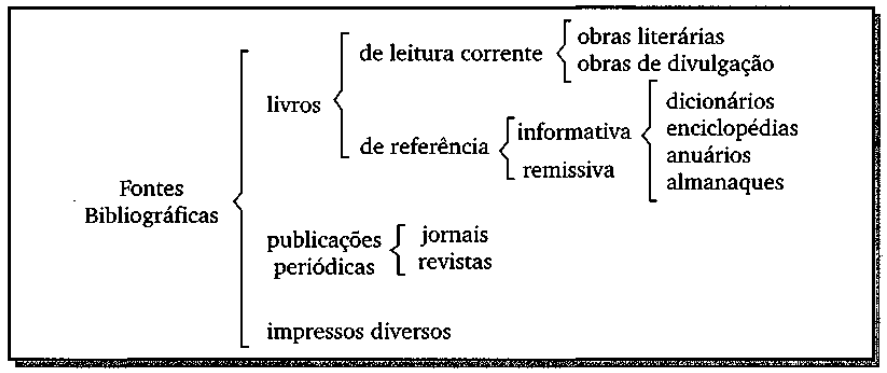
\includegraphics[keepaspectratio=true,scale=0.3]{figuras/tiposDePesquisaBibliografica.png}
\caption{Classificação das pesquisas bibliográficas}
\label{tiposDePesquisaBibliografica}
\end{figure}
	
	Os livros são fontes bibliográficas de excelência, classificados como de leitura corrente ou de referência. Os livros de literatura corrente são aqueles que objetivam conferir conhecimentos científicos ou técnicos ao leitor, já os de referência tem por objetivo proporcionar ao leitor a rápida obtenção das informações requeridas (informativa) ou a referência às obras que as contenham (remissiva) \cite{ac2002elaborar}.  
A pesquisa bibliográfica é muito vantajosa ao pesquisador, já que este pode ter acesso a uma gama de informações muito maior do que aquelas que ele conseguiria pesquisando diretamente. Essa pesquisa também é de suma importância na pesquisas históricas, pois a maioria dos fatos só é possível conhecer por esse tipo de pesquisa.
A desvantagem dessa pesquisa é a possível propagação de erro, pois que a fonte bibliográfica utilizada estiver com algum dado equivocado, este será refletido no trabalho do pesquisador.	
\subsubsection{Pesquisa Documental}
A pesquisa documental é difícil de distinguir da pesquisa bibliográfica, pois ambas utilizam material impresso para um determinado público como fonte de pesquisa. A principal divergência que pode-se destacar é quanto ao tratamento análitico das fontes. A pesquisa documental utiliza fontes de pesquisa que não passaram por um tratamento análitico, ou seja, são matéria-prima como cartas pessoais, fotos, diários, memorandos e outros, a partir da qual o pesquisador vai desenvolver a sua pesquisa. A pesquisa bibliográfica se utiliza de fontes de pesquisas já analisadas como livros e periódicos \cite{ac2002elaborar}.
\subsubsection{Pesquisa Experimental}
A pesquisa experimental consiste em determinar o objeto de estudo, as possíveis variáveis capazes de influência-lo, as formas de controle e observação dos efeitos, fazendo com que o pesquisador seja o agente ativo da pesquisa. Uma pesquisa experimental pode ser desevolvida em qualquer lugar, desde que ela possa ser manipulada e controlada pelo pesquisador e que haja uma distribuição aleatória dos elementos que iram participar do experimento. As pesquisas experiamentais são as mais utilizadas para se provar hipóteses de causa-efeito, porém é um ambiente com variáveis controladas, logo, pode haver variáveis de difícil controle ou até mesmo impossível tornando o experimento inviável. \cite{ac2002elaborar}
\subsubsection{Pesquisa \textit{Ex-post Facto}}
A tradução literal de \textit{ex-post facto} é "de um fato passado", ou seja, a pesquisa \textit{ex-post facto} é realizada após a ocorrência de variáveis no objeto de estudo. A diferença entre a pesquisa \textit{ex-post facto} e a pesquisa experimental é que esta verifica a causa-efeito com o controle de variáveis, enquanto aquela verifica a causa-efeito sem o controle de variáveis, já que o fato já ocorreu. Esse tipo de pesquisa é muitas vezes chamada de correlacional, pois nela é possível se identificar a existência de relação entre variáveis. \cite{ac2002elaborar}
\subsubsection{Levantamento}
O levantamento é utilizado quando se interroga diretamente as pessoas que se quer conhecer o comportamento, procura ser representativo de universo definido, identificando as características dos componentes desse universo e oferecer resultados pela precisão estática, através da caracterização dos segmentos. Um questionário pode ser utilizado para coletar os dados, e depois é feita a análise quantitativa dessa coleta. Quando um levantamento é feito sobre um grupo muito grande de pessoas este é chamado de "censo". \cite{prodanov2013metodologia} 	
\subsubsection{Estudo de Caso}
O estudo de caso busca o aprofundamento nas questões propostas, estudando um único grupo ou comunidade, utilizando mais a observação direta do que a interrogação, captando as explicações e interpretações do que ocorre no grupo. No estudo de campo, o pesquisador está inserido no grupo, para poder entender melhor as regras, os costumes e as conveções.

\section{Planejamento da pesquisa}
O modelo híbrido de pesquisa exploratório/experimental será utilizado nesse TCC para avaliar os vários tipos de algoritmos que podem ser utilizados como solução para a questão de pesquisa. Após a escolha do algoritmo ter sido feita, este será adaptado ao contexto do LEGO Mindstorms, utilizando o modelo híbrido de pesquisa exploratório/descritivo.
Pretende-se ainda, nas atividades específicas de desenvolvimento, fazer uso de uma  metodologia orientada aos princípios ágeis, uma possível adaptação do Scrum, com sprints
de uma semana (em média), as quais ocorrerão em ambiente controlado e terão seus resultados quantificados.
Dado que a pesquisa será exploratória/experimental e exploratória/descritiva, muito provavelmente será utilizado o modelo de pesquisa-ação ao longo do projeto. Esse modelo permitirá, dentre outras contribuições, a retroalimentação da solução com base nos experimentos realizados ao longo da condução do trabalho.

\section{Modelagem da metodologia}
Com intuito de ilustrar como será realizada a condução deste projeto, segue a
Figura \ref{modelagem} que apresenta a modelagem do processo metodológico com base na metodologia
descrita nesta seção.

\FloatBarrier
\begin{figure}[!h]
\centering
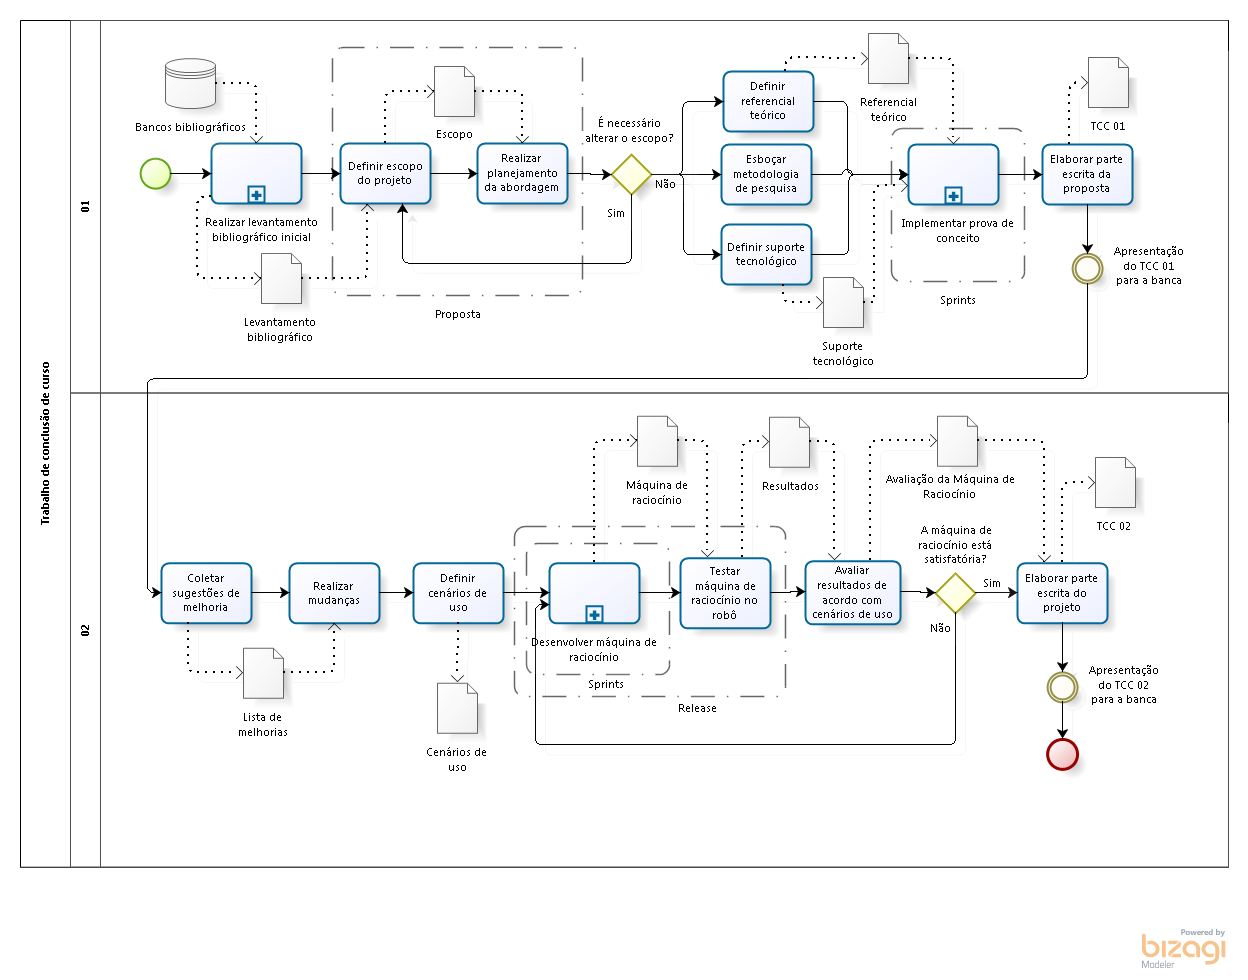
\includegraphics[keepaspectratio=true,scale=0.5]{figuras/modelagemTcc.png}
\caption{Modelagem do processo utilizado no TCC}
\label{modelagem}
\end{figure}
\clearpage
 
\section{Cronograma da pesquisa}
O cronograma, detalhado nas Tabelas \ref{tab01} e \ref{tab02}, visa conferir uma noção temporal acerca das atividades definidas para o processo. Trata-se de uma visão preliminar, logo, pode haver modificações ao longo do projeto de acordo com as necessidades.      

\FloatBarrier
\begin{table}[h]
	\centering
	
	\begin{tabular}{lcccccc}
		\toprule
		& \textbf{Jan} & \textbf{Fev} & \textbf{Mar} & \textbf{Abr} & \textbf{Mai} & 		
		\textbf{Jun} \\
		\midrule
		Realizar levantamento bibliográfico inicial & X & X &  &  &  &  \\
		\midrule
		Definir escopo do projeto &  & X &  &  &  &  \\
		\midrule
		Realizar planejamento da abordagem &  &  & X &  &  &  \\
		\midrule
		Definir referencial teórico &  &  &  & X & X &  \\
		\midrule
		Definir suporte tecnológico &  &  &  & X & X &  \\
		\midrule
		Esboçar metodologia de pesquisa &  &  &  & X & X &  \\
		\midrule
		Implementar prova de conceito &  &  &  &  &  & X \\
		\midrule
		Elaborar parte escrita da proposta &  &  &  &  &  & X \\
		\bottomrule
	\end{tabular}

	\caption{Cronograma do TCC 01}
	\label{tab01}
\end{table}

\FloatBarrier
\begin{table}[h]
	\centering
	
	\begin{tabular}{lcccccc}
		\toprule
		& \textbf{Jul} & \textbf{Ago} & \textbf{Set} & \textbf{Out} & \textbf{Nov} & 		
		\textbf{Dez} \\
		\midrule
		Coletar sugestões de melhoria & X &  &  &  &  &  \\
		\midrule
		Realizar mudanças & X &  &  &  &  &  \\
		\midrule
		Definir cenários de uso & X &  &  &  &  &  \\
		\midrule
		Desenvolver máquina de racionício &  & X & X & X &  &  \\
		\midrule
		Testar máquina de raciocínio no robô &  &  & X & X &  &  \\
		\midrule
		Avaliar resultados de acordo com cenários de uso &  &  & X & X &  &  \\
		\midrule
		Elaborar parte escrita do projeto &  &  &  &  & X &  \\
		\bottomrule
	\end{tabular}

	\caption{Cronograma do TCC 02}
	\label{tab02}
\end{table}
\section{Considerações finais}